\documentclass[]{article}
\usepackage{lmodern}
\usepackage{amssymb,amsmath}
\usepackage{ifxetex,ifluatex}
\usepackage{fixltx2e} % provides \textsubscript
\ifnum 0\ifxetex 1\fi\ifluatex 1\fi=0 % if pdftex
  \usepackage[T1]{fontenc}
  \usepackage[utf8]{inputenc}
\else % if luatex or xelatex
  \ifxetex
    \usepackage{mathspec}
  \else
    \usepackage{fontspec}
  \fi
  \defaultfontfeatures{Ligatures=TeX,Scale=MatchLowercase}
\fi
% use upquote if available, for straight quotes in verbatim environments
\IfFileExists{upquote.sty}{\usepackage{upquote}}{}
% use microtype if available
\IfFileExists{microtype.sty}{%
\usepackage{microtype}
\UseMicrotypeSet[protrusion]{basicmath} % disable protrusion for tt fonts
}{}
\usepackage[margin=1in]{geometry}
\usepackage{hyperref}
\hypersetup{unicode=true,
            pdfborder={0 0 0},
            breaklinks=true}
\urlstyle{same}  % don't use monospace font for urls
\usepackage{graphicx}
% grffile has become a legacy package: https://ctan.org/pkg/grffile
\IfFileExists{grffile.sty}{%
\usepackage{grffile}
}{}
\makeatletter
\def\maxwidth{\ifdim\Gin@nat@width>\linewidth\linewidth\else\Gin@nat@width\fi}
\def\maxheight{\ifdim\Gin@nat@height>\textheight\textheight\else\Gin@nat@height\fi}
\makeatother
% Scale images if necessary, so that they will not overflow the page
% margins by default, and it is still possible to overwrite the defaults
% using explicit options in \includegraphics[width, height, ...]{}
\setkeys{Gin}{width=\maxwidth,height=\maxheight,keepaspectratio}
\IfFileExists{parskip.sty}{%
\usepackage{parskip}
}{% else
\setlength{\parindent}{0pt}
\setlength{\parskip}{6pt plus 2pt minus 1pt}
}
\setlength{\emergencystretch}{3em}  % prevent overfull lines
\providecommand{\tightlist}{%
  \setlength{\itemsep}{0pt}\setlength{\parskip}{0pt}}
\setcounter{secnumdepth}{0}
% Redefines (sub)paragraphs to behave more like sections
\ifx\paragraph\undefined\else
\let\oldparagraph\paragraph
\renewcommand{\paragraph}[1]{\oldparagraph{#1}\mbox{}}
\fi
\ifx\subparagraph\undefined\else
\let\oldsubparagraph\subparagraph
\renewcommand{\subparagraph}[1]{\oldsubparagraph{#1}\mbox{}}
\fi

%%% Use protect on footnotes to avoid problems with footnotes in titles
\let\rmarkdownfootnote\footnote%
\def\footnote{\protect\rmarkdownfootnote}

%%% Change title format to be more compact
\usepackage{titling}

% Create subtitle command for use in maketitle
\providecommand{\subtitle}[1]{
  \posttitle{
    \begin{center}\large#1\end{center}
    }
}

\setlength{\droptitle}{-2em}

  \title{}
    \pretitle{\vspace{\droptitle}}
  \posttitle{}
    \author{}
    \preauthor{}\postauthor{}
    \date{}
    \predate{}\postdate{}
  

\begin{document}

\hypertarget{red-wine-quality-analysis-by-mohamed_alsayed}{%
\section{Red Wine Quality Analysis by
Mohamed\_Alsayed}\label{red-wine-quality-analysis-by-mohamed_alsayed}}

\begin{quote}
This tidy data set contains 1,599 red wines with 11 variables on the
chemical properties of the wine. At least 3 wine experts rated the
quality of each wine, providing a rating between 0 (very bad) and 10
(very excellent).
\end{quote}

\hypertarget{univariate-plots-section}{%
\section{Univariate Plots Section}\label{univariate-plots-section}}

\begin{verbatim}
##    Min. 1st Qu.  Median    Mean 3rd Qu.    Max. 
##   3.000   5.000   6.000   5.636   6.000   8.000
\end{verbatim}

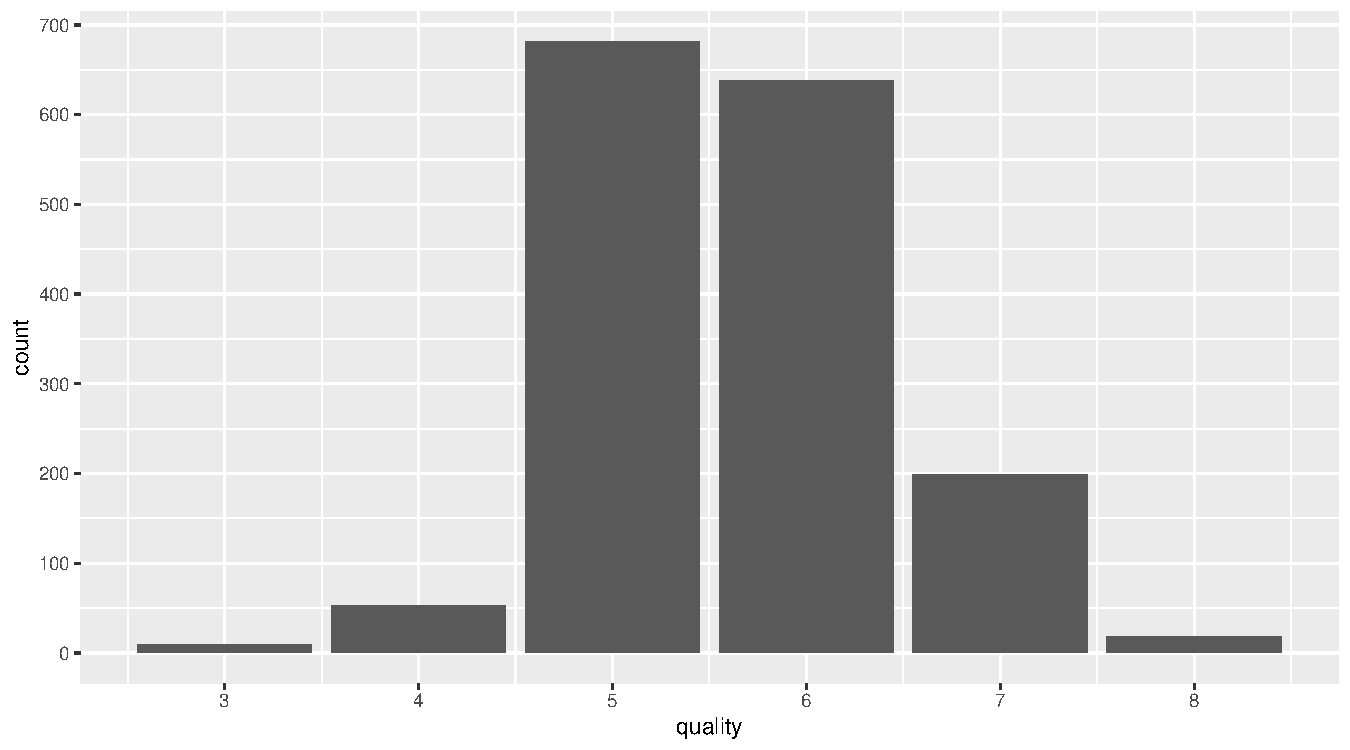
\includegraphics{RedWineQuality-Project6_files/figure-latex/Univariate_Plots-1.pdf}

\begin{quote}
The quality histogram shows that the majority of wine samples are rated
5 or 6 while few samples are rated 1 and 8 and no sample rated above 8
nor less than 3.
\end{quote}

\begin{verbatim}
##    Min. 1st Qu.  Median    Mean 3rd Qu.    Max. 
##    4.60    7.10    7.90    8.32    9.20   15.90
\end{verbatim}

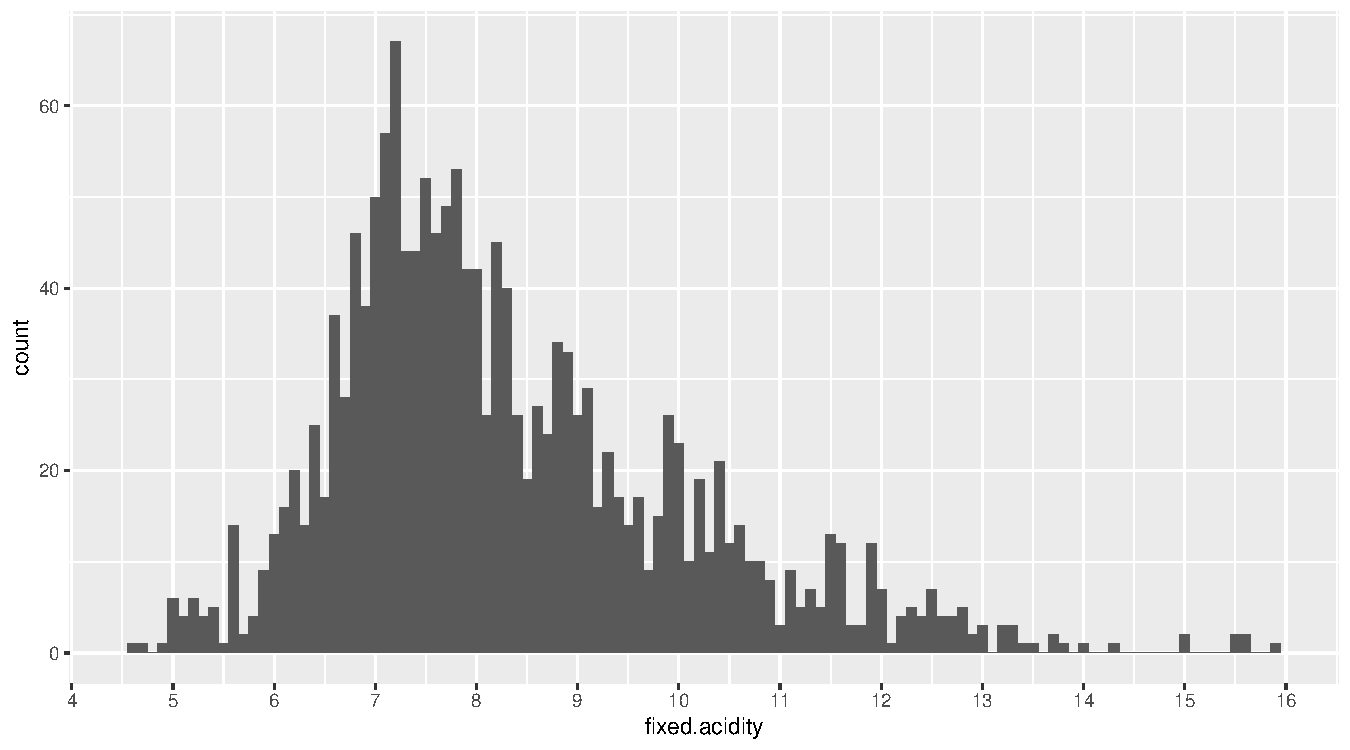
\includegraphics{RedWineQuality-Project6_files/figure-latex/unnamed-chunk-1-1.pdf}

\begin{quote}
The fixed acidity histogram show that the majority of wine samples has
fixed acidity of apporximately 7 to 8 and the rest ranges between 4.5 to
13 and few of the samples has higher fixed acidity above 13 to 16.
\end{quote}

\begin{verbatim}
##    Min. 1st Qu.  Median    Mean 3rd Qu.    Max. 
##  0.1200  0.3900  0.5200  0.5278  0.6400  1.5800
\end{verbatim}

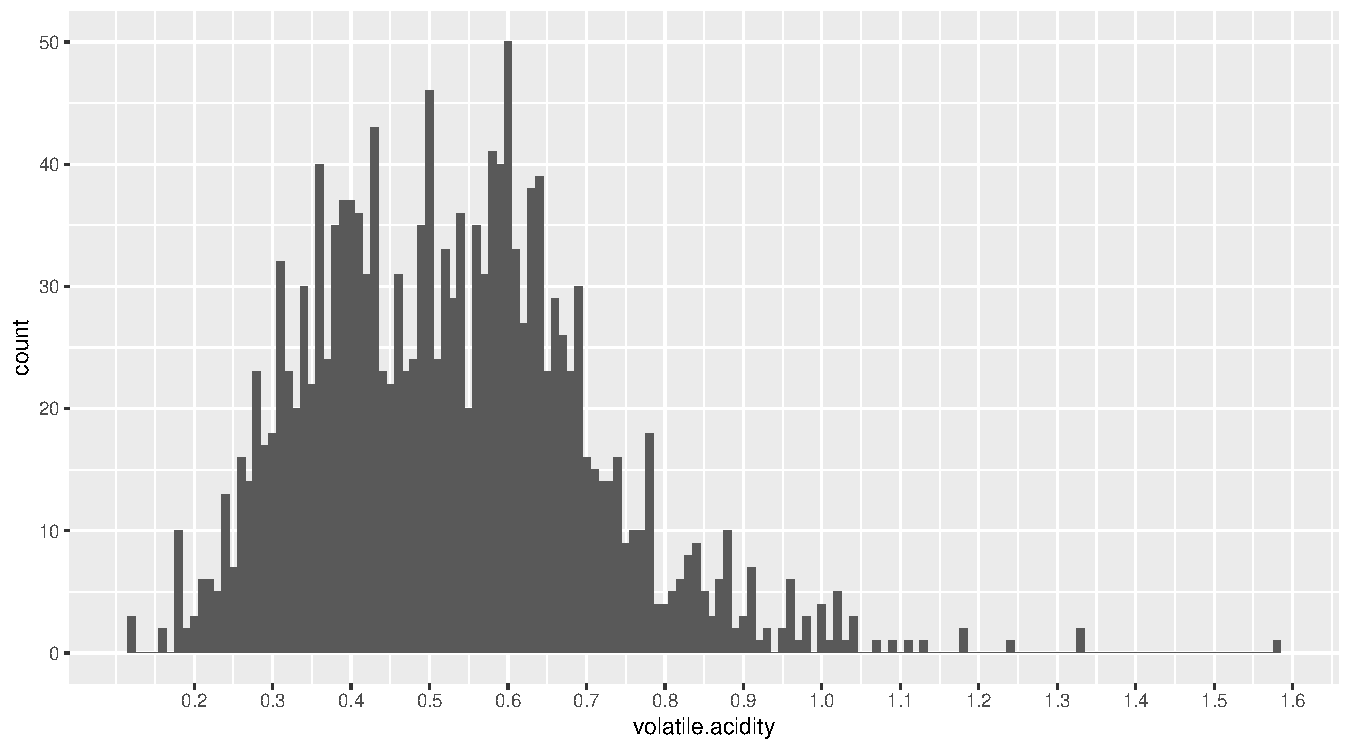
\includegraphics{RedWineQuality-Project6_files/figure-latex/unnamed-chunk-2-1.pdf}

\begin{quote}
The volatile acidity histogram show that the majority of wine samples
has volatile acidity of 0.3 to 0.7
\end{quote}

\begin{verbatim}
##    Min. 1st Qu.  Median    Mean 3rd Qu.    Max. 
##   0.000   0.090   0.260   0.271   0.420   1.000
\end{verbatim}

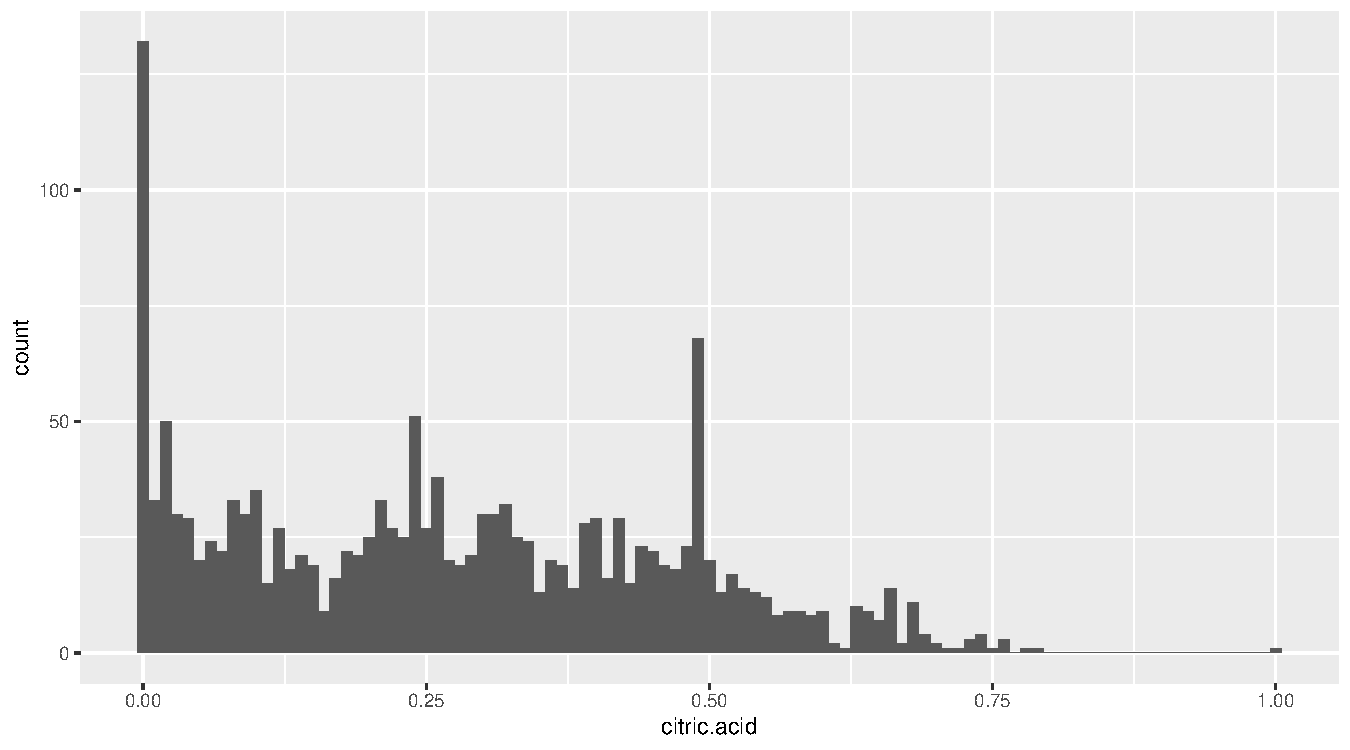
\includegraphics{RedWineQuality-Project6_files/figure-latex/unnamed-chunk-3-1.pdf}

\begin{quote}
The Citric Acid histogram shows that the majority of wine samples ranges
between 0 and 0.75 and also we can observe high number of these samples
has 0 citric acid as well as 0.5 citric acid.
\end{quote}

\begin{verbatim}
##    Min. 1st Qu.  Median    Mean 3rd Qu.    Max. 
##   0.900   1.900   2.200   2.539   2.600  15.500
\end{verbatim}

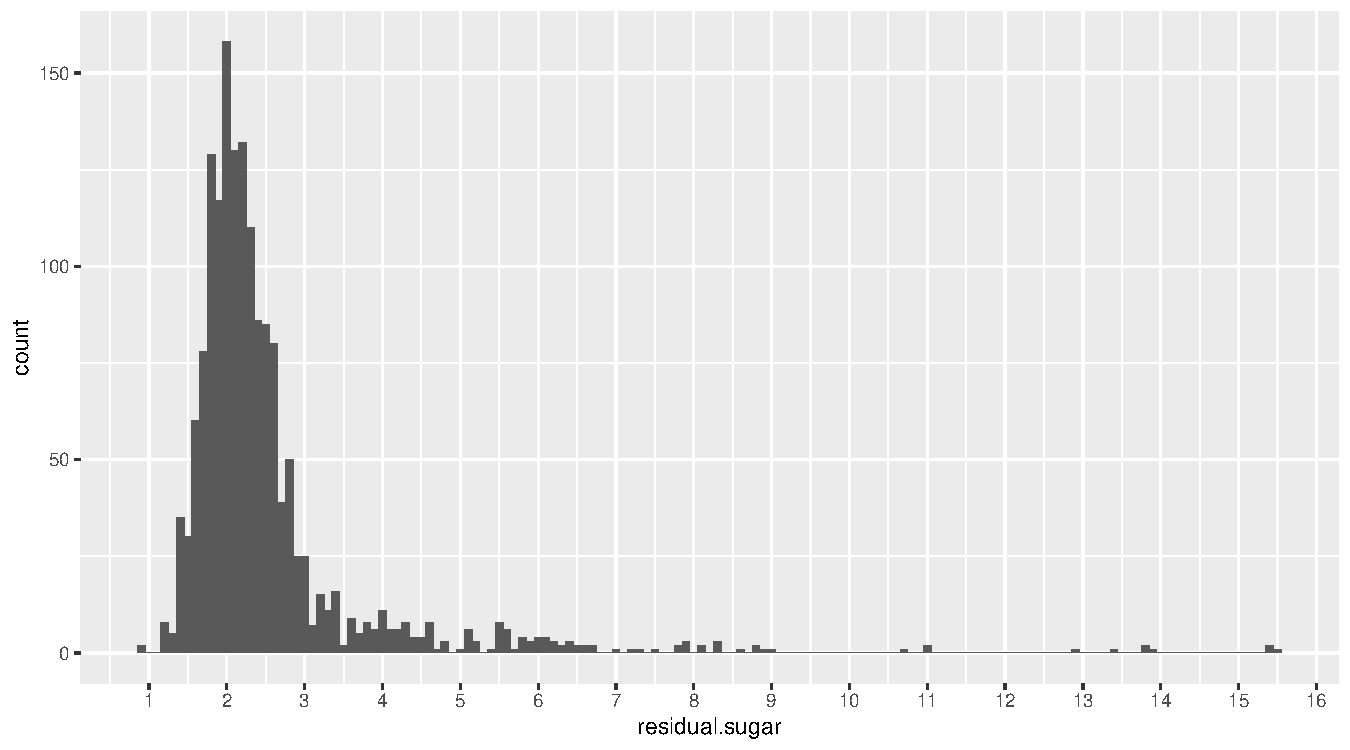
\includegraphics{RedWineQuality-Project6_files/figure-latex/unnamed-chunk-4-1.pdf}

\begin{quote}
The Residual Sugar histogram shows that most of wine samples are between
2 and 3 on residual sugar and some few samples above 4 to 16.
\end{quote}

\begin{verbatim}
##    Min. 1st Qu.  Median    Mean 3rd Qu.    Max. 
## 0.01200 0.07000 0.07900 0.08747 0.09000 0.61100
\end{verbatim}

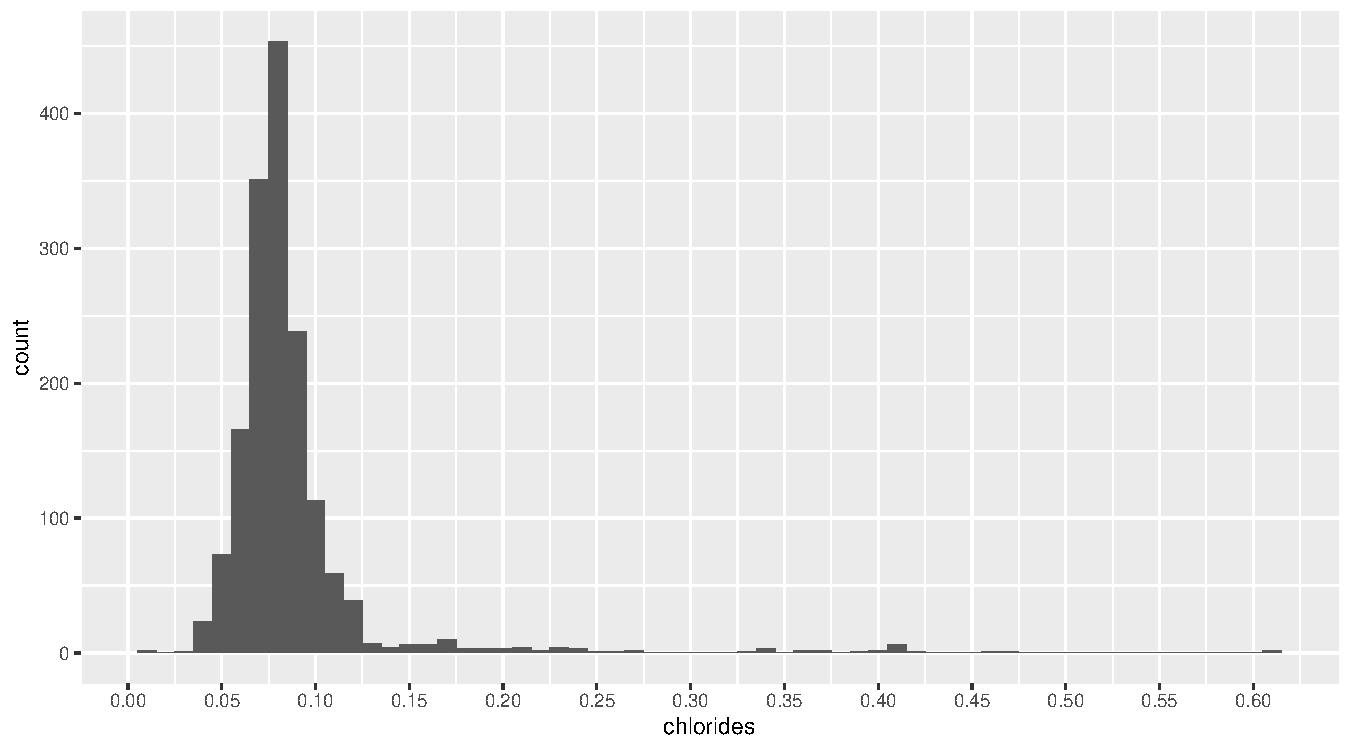
\includegraphics{RedWineQuality-Project6_files/figure-latex/unnamed-chunk-5-1.pdf}
\textgreater The Chlorides histogram shows that the majority of wine
samples are between 0.05 to 0.1 on the chlorides scale.

\begin{verbatim}
##    Min. 1st Qu.  Median    Mean 3rd Qu.    Max. 
##    1.00    7.00   14.00   15.87   21.00   72.00
\end{verbatim}

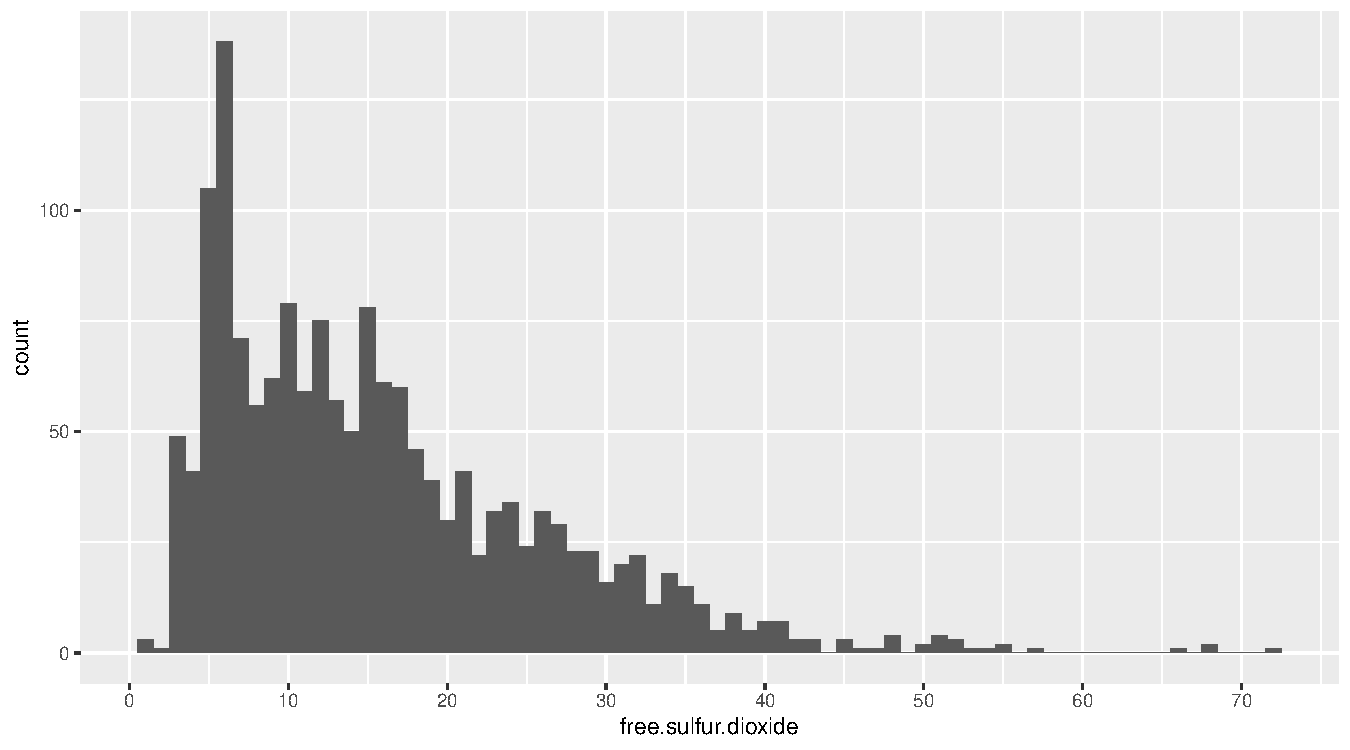
\includegraphics{RedWineQuality-Project6_files/figure-latex/unnamed-chunk-6-1.pdf}

\begin{quote}
The Free Sulfur Dioxide histogram shows that the wine samples ranges
between 0 to 50 and many samples has 5 value on the free sulfur dioxide
scale.
\end{quote}

\begin{verbatim}
##    Min. 1st Qu.  Median    Mean 3rd Qu.    Max. 
##    6.00   22.00   38.00   46.47   62.00  289.00
\end{verbatim}

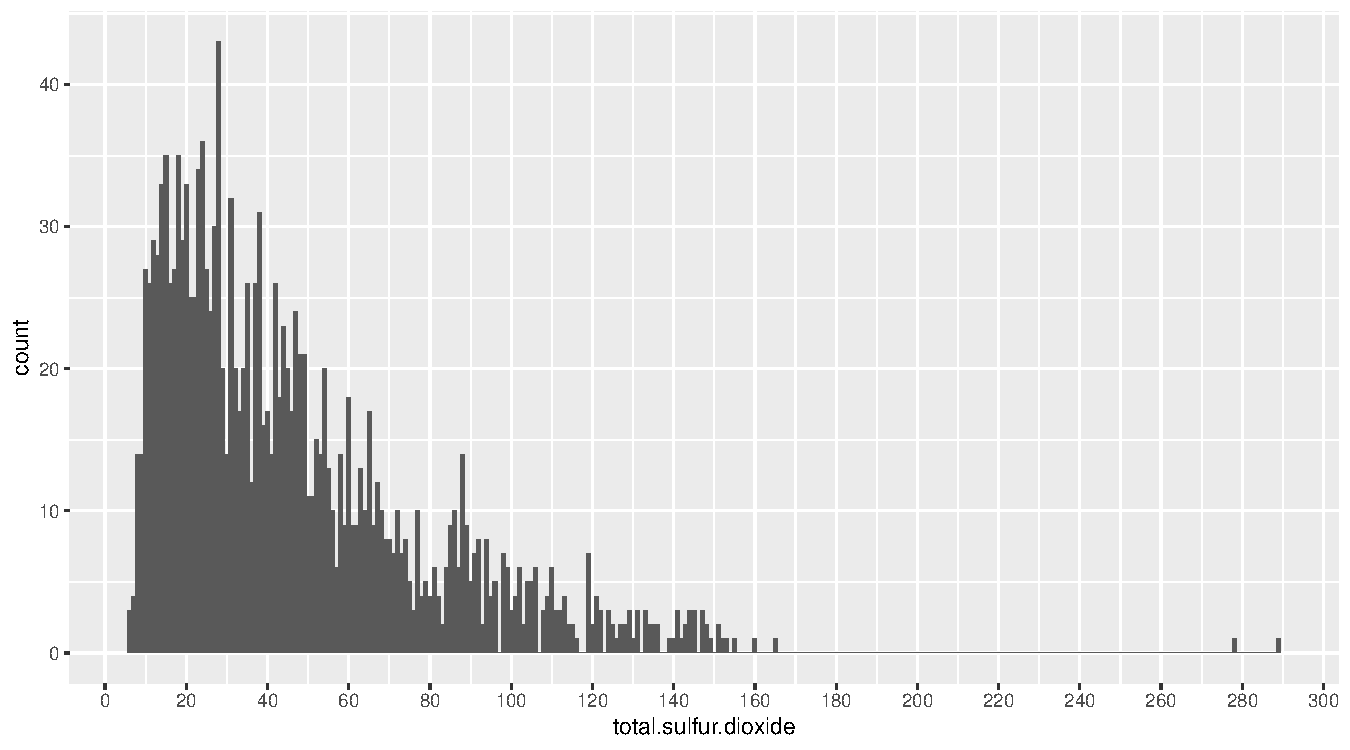
\includegraphics{RedWineQuality-Project6_files/figure-latex/unnamed-chunk-7-1.pdf}
\textgreater The total Sulfur Dioxide histogram shows that the majority
of wine samples ranges between 10 to 120 and there are some outliers
above 260 .

\begin{verbatim}
##    Min. 1st Qu.  Median    Mean 3rd Qu.    Max. 
##  0.9901  0.9956  0.9968  0.9967  0.9978  1.0037
\end{verbatim}

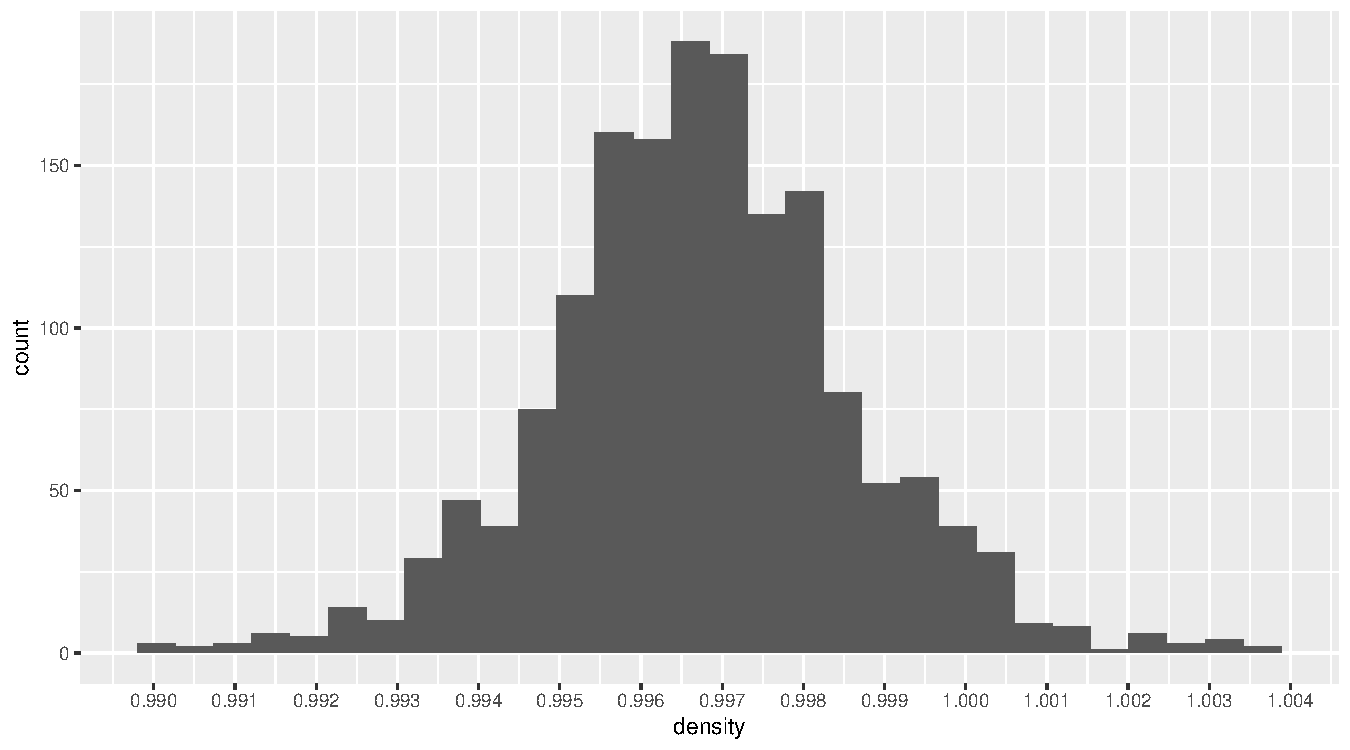
\includegraphics{RedWineQuality-Project6_files/figure-latex/unnamed-chunk-8-1.pdf}

\begin{quote}
The density histogram shows a nearly normal distrbuted data with a peak
of 0.997 and range between 0.990 to 1.004
\end{quote}

\begin{verbatim}
##    Min. 1st Qu.  Median    Mean 3rd Qu.    Max. 
##   2.740   3.210   3.310   3.311   3.400   4.010
\end{verbatim}

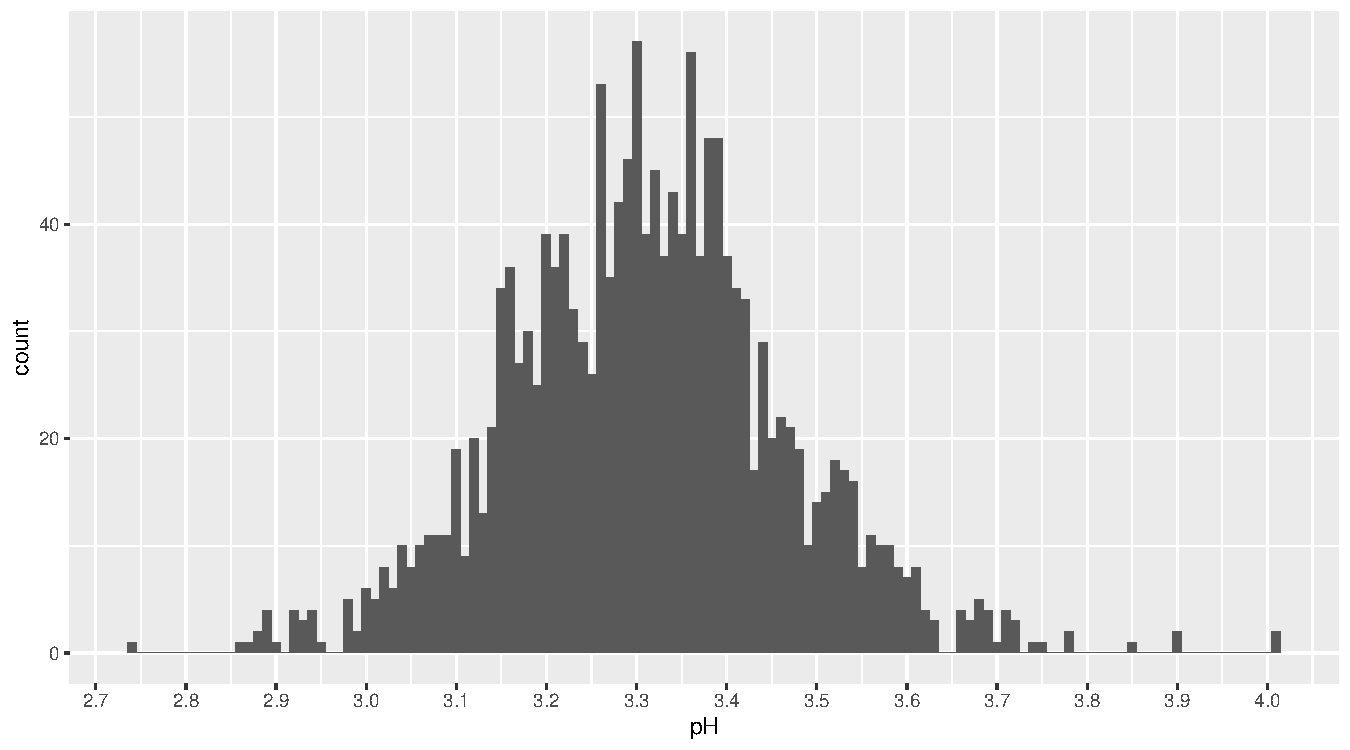
\includegraphics{RedWineQuality-Project6_files/figure-latex/unnamed-chunk-9-1.pdf}

\begin{quote}
The Ph histogram shows that most wine sample has ph value that ranges
between 3 to 3.7 and some of the outlier samples are above 4.
\end{quote}

\begin{verbatim}
##    Min. 1st Qu.  Median    Mean 3rd Qu.    Max. 
##  0.3300  0.5500  0.6200  0.6581  0.7300  2.0000
\end{verbatim}

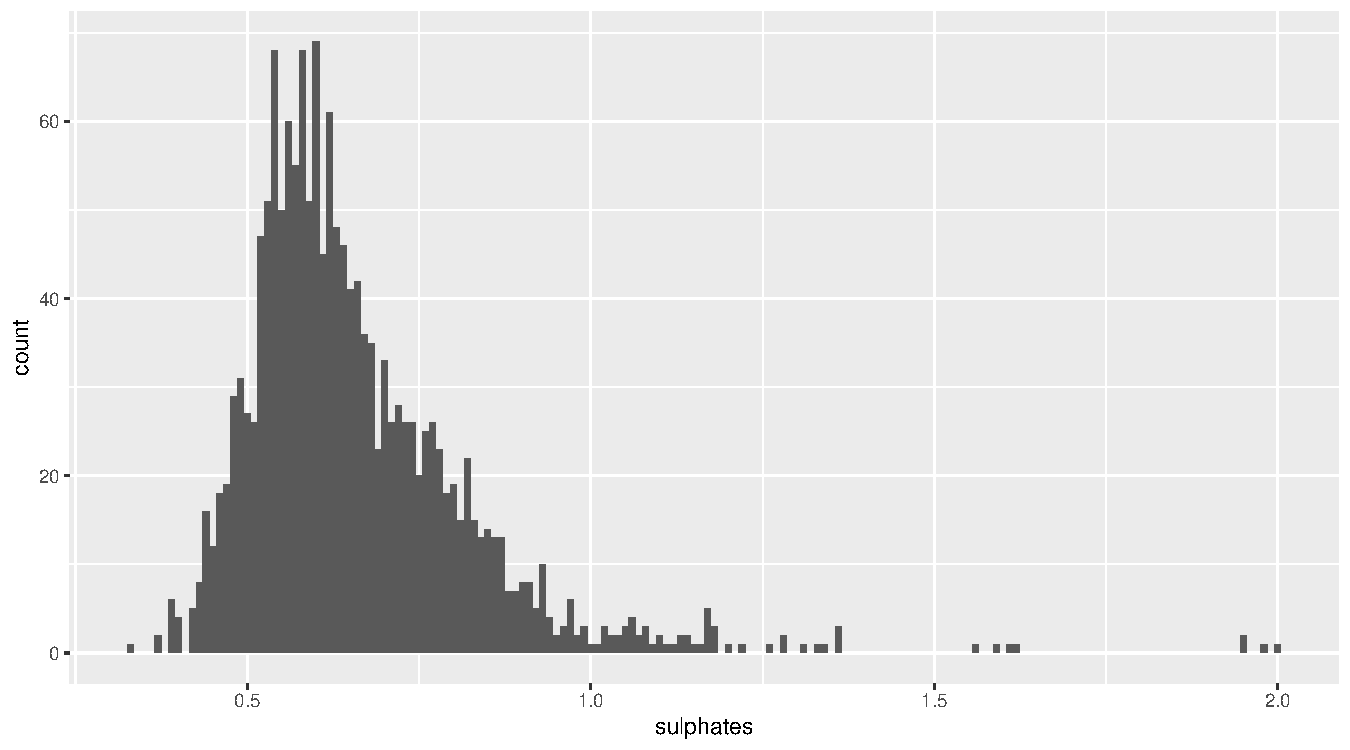
\includegraphics{RedWineQuality-Project6_files/figure-latex/unnamed-chunk-10-1.pdf}

\begin{quote}
The sulphates histogram shows that most of wine samples are ranging
between 0.5 to 1.
\end{quote}

\begin{verbatim}
##    Min. 1st Qu.  Median    Mean 3rd Qu.    Max. 
##    8.40    9.50   10.20   10.42   11.10   14.90
\end{verbatim}

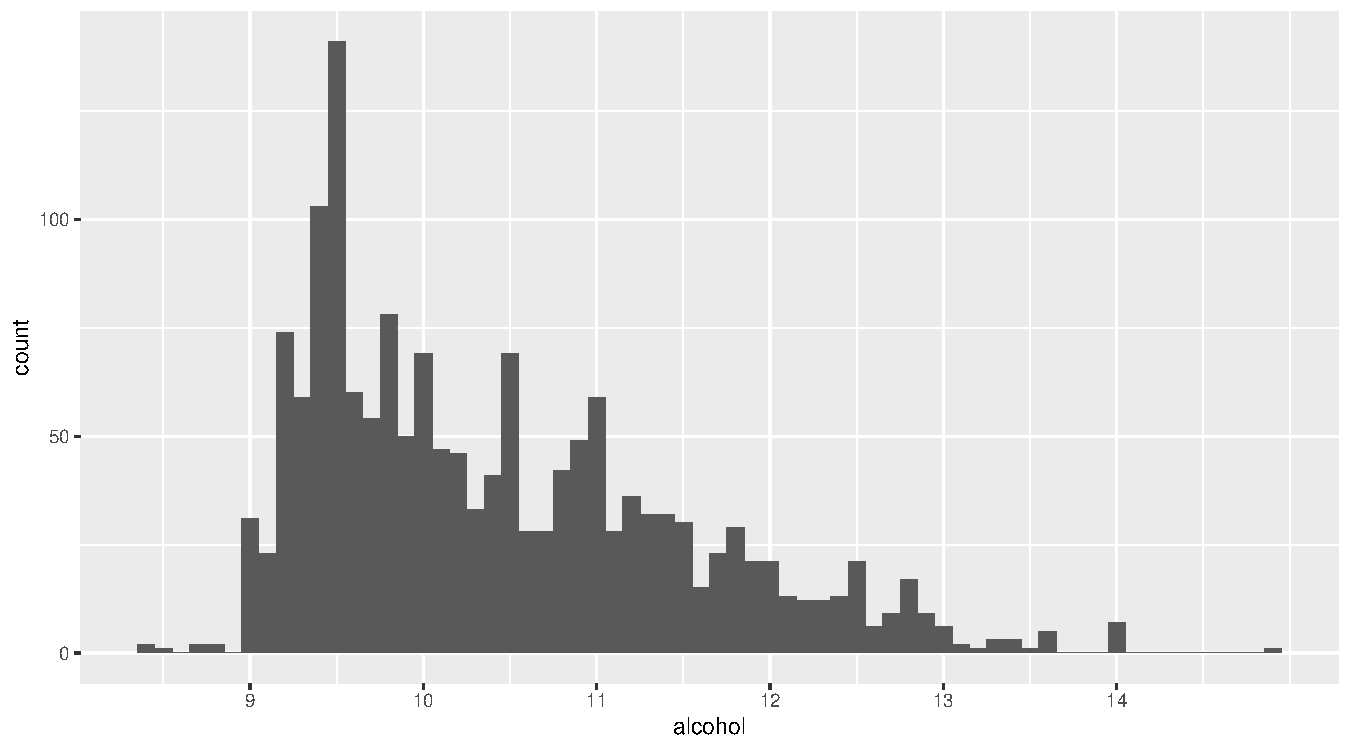
\includegraphics{RedWineQuality-Project6_files/figure-latex/unnamed-chunk-11-1.pdf}

\begin{quote}
The Alcohol histogram shows that the wine samples has alcohol ranges
between 9 to 14 with a high number of samples contains 9.5 of alcohol.
\end{quote}

\hypertarget{univariate-analysis}{%
\section{Univariate Analysis}\label{univariate-analysis}}

\hypertarget{what-is-the-structure-of-your-dataset}{%
\subsubsection{What is the structure of your
dataset?}\label{what-is-the-structure-of-your-dataset}}

The dataset consist of 11 variables that contribute in the red wine
quality like alcohol, ph and density.

\hypertarget{what-isare-the-main-features-of-interest-in-your-dataset}{%
\subsubsection{What is/are the main feature(s) of interest in your
dataset?}\label{what-isare-the-main-features-of-interest-in-your-dataset}}

The most interesting variable is alcohol since its the main factor
contributing directly to the quality of the red wine.

\hypertarget{what-other-features-in-the-dataset-do-you-think-will-help-support-your}{%
\subsubsection{\texorpdfstring{What other features in the dataset do you
think will help support your\\
}{What other features in the dataset do you think will help support your }}\label{what-other-features-in-the-dataset-do-you-think-will-help-support-your}}

investigation into your feature(s) of interest? The ph value as well as
the density of the wine will both be good factors to detrmine the wine
quality.

\hypertarget{did-you-create-any-new-variables-from-existing-variables-in-the-dataset}{%
\subsubsection{Did you create any new variables from existing variables
in the
dataset?}\label{did-you-create-any-new-variables-from-existing-variables-in-the-dataset}}

I measured every variable independently to be able to see its effect on
the quality and no new variables has been added.

\hypertarget{of-the-features-you-investigated-were-there-any-unusual-distributions}{%
\subsubsection{\texorpdfstring{Of the features you investigated, were
there any unusual distributions?\\
}{Of the features you investigated, were there any unusual distributions? }}\label{of-the-features-you-investigated-were-there-any-unusual-distributions}}

Did you perform any operations on the data to tidy, adjust, or change
the form\\
of the data? If so, why did you do this? The data is pretty tidy and has
no errors nor nulls but distributions just needed some adjustment for
readability so I changed the bin width for most of histograms and
adjusted their axis for better observations.

\hypertarget{bivariate-plots-section}{%
\section{Bivariate Plots Section}\label{bivariate-plots-section}}

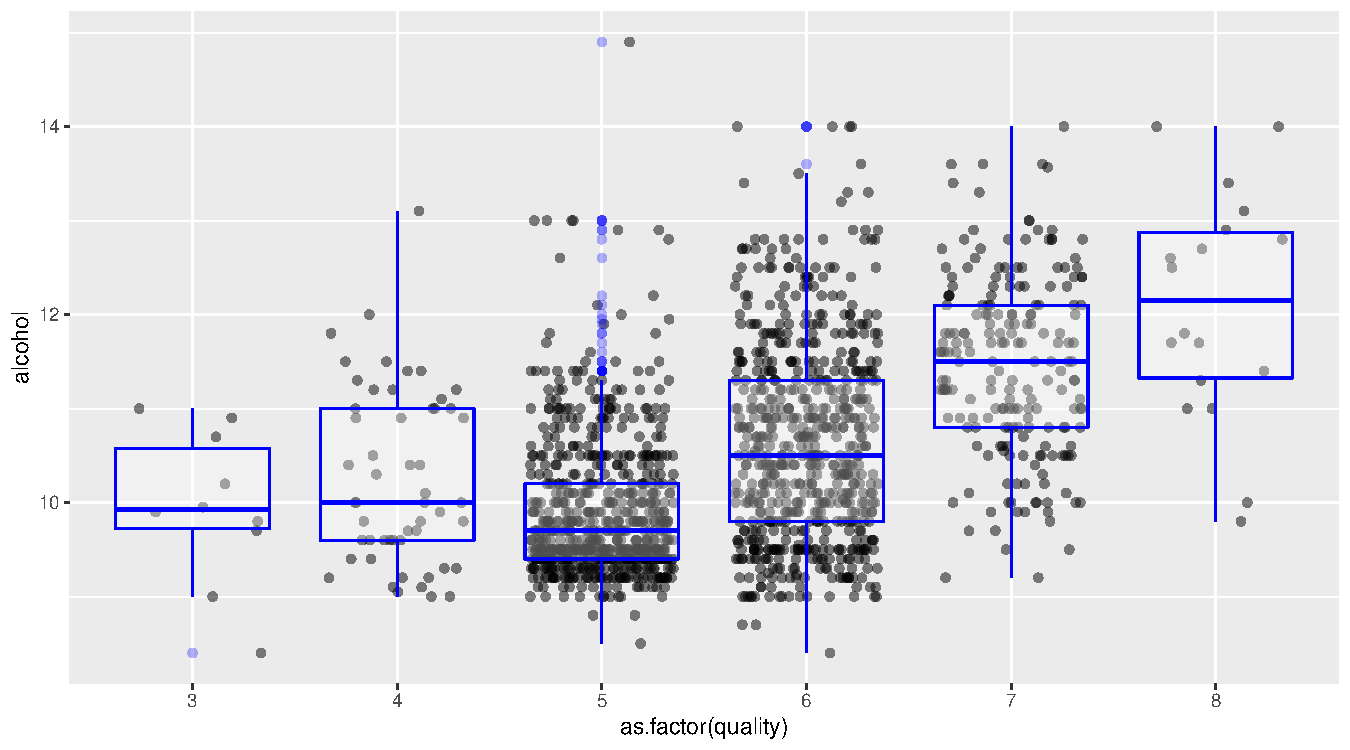
\includegraphics{RedWineQuality-Project6_files/figure-latex/Bivariate_Plots-1.pdf}

\begin{quote}
The plot above shows the relation between alcohol and the quality of red
wine, and we can observe that the quality increases when alcohol
increases.
\end{quote}

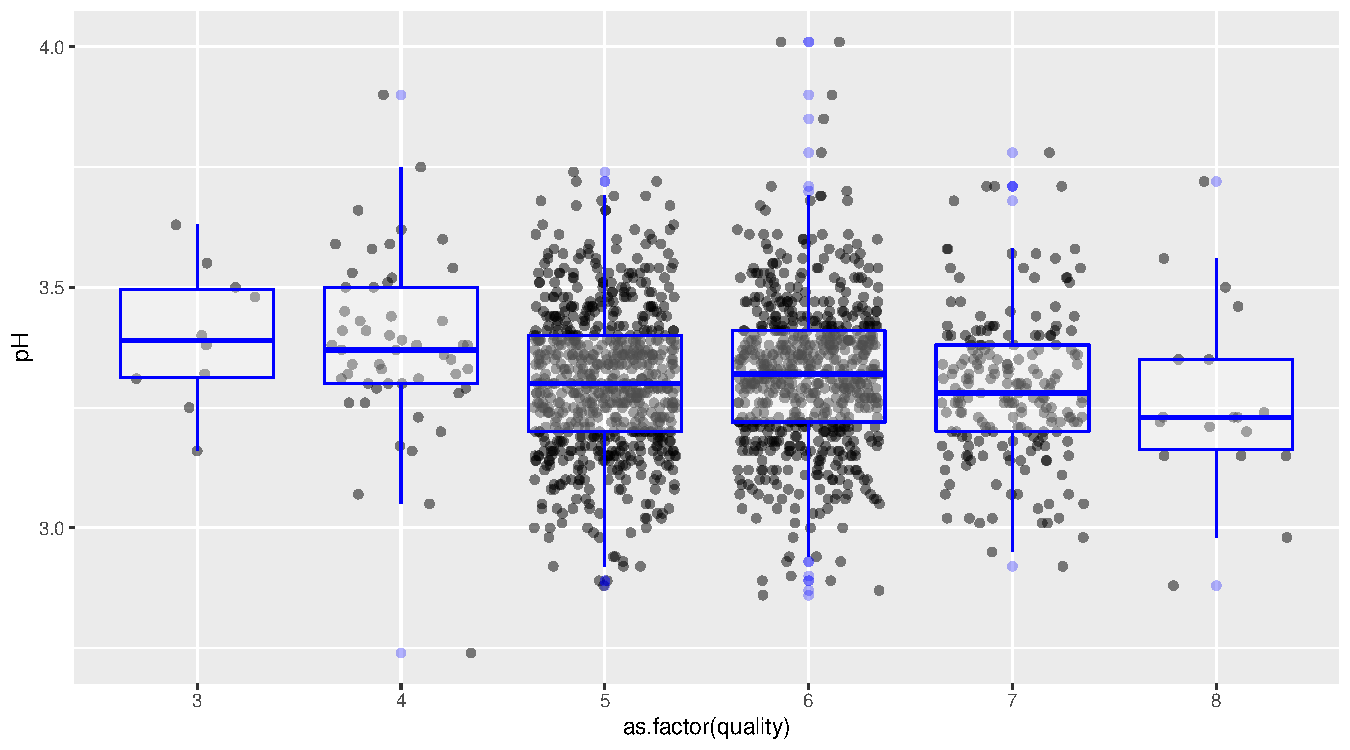
\includegraphics{RedWineQuality-Project6_files/figure-latex/unnamed-chunk-12-1.pdf}

\begin{quote}
The relation between pH and the quality are week and the plot shows that
high pH can get nearly same result as lower pH in quality.
\end{quote}

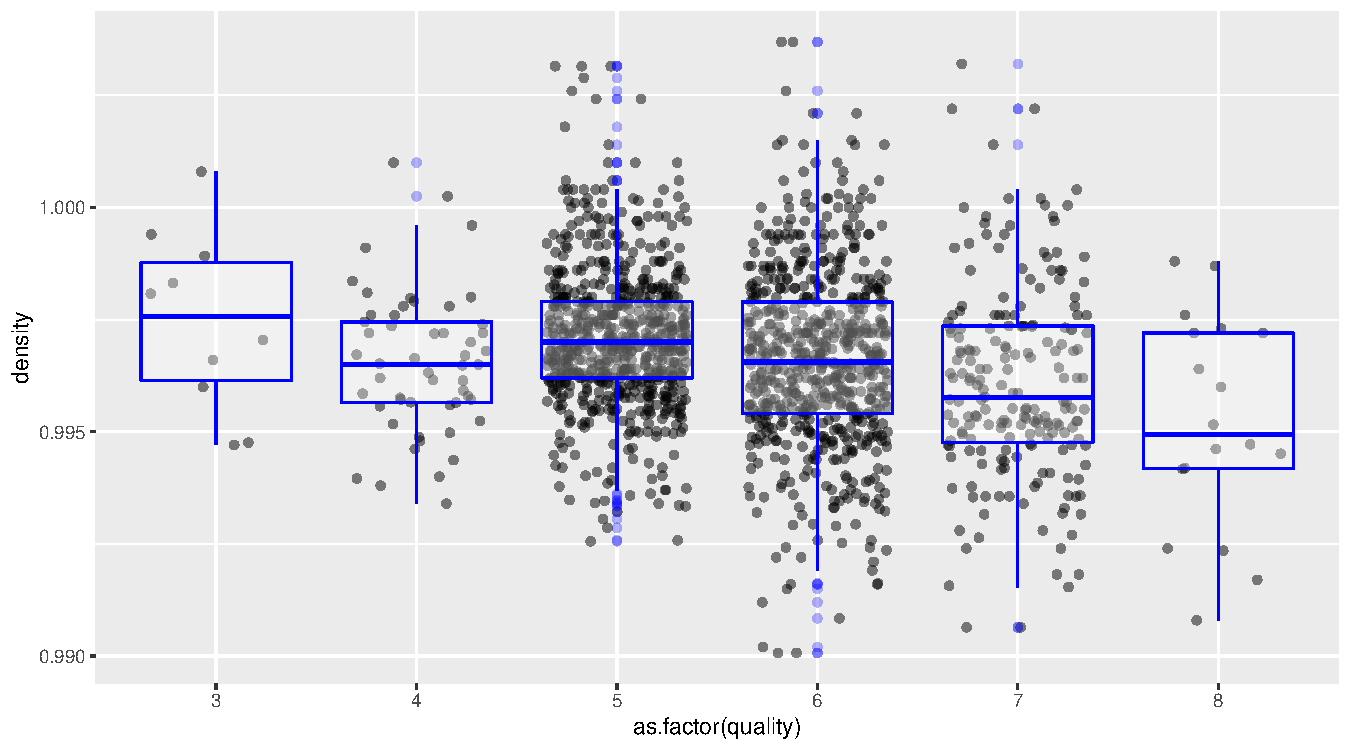
\includegraphics{RedWineQuality-Project6_files/figure-latex/unnamed-chunk-13-1.pdf}

\begin{quote}
The plot above showing the relation between quality and density, we can
observe that there is an inverse relation when density increases the
quality decreases and vice versa.
\end{quote}

\hypertarget{bivariate-analysis}{%
\section{Bivariate Analysis}\label{bivariate-analysis}}

\hypertarget{talk-about-some-of-the-relationships-you-observed-in-this-part-of-the}{%
\subsubsection{\texorpdfstring{Talk about some of the relationships you
observed in this part of the\\
}{Talk about some of the relationships you observed in this part of the }}\label{talk-about-some-of-the-relationships-you-observed-in-this-part-of-the}}

investigation. How did the feature(s) of interest vary with other
features in\\
the dataset?

-Alcholol has big impact on the quality level of the red wine, we can
see from the plotted data that the increase of alchohol increases the
chance of high quality rates. -Density has inverse relation with the
quality when the density increases the quality decreases -The pH value
of the red wine did not show much relation and effect on the quality
rate of the red wine.

\hypertarget{did-you-observe-any-interesting-relationships-between-the-other-features}{%
\subsubsection{\texorpdfstring{Did you observe any interesting
relationships between the other features\\
}{Did you observe any interesting relationships between the other features }}\label{did-you-observe-any-interesting-relationships-between-the-other-features}}

(not the main feature(s) of interest)?

Yes, both density and pH values and how both impacted the change in
quality rates across all red wine samples.

\hypertarget{what-was-the-strongest-relationship-you-found}{%
\subsubsection{What was the strongest relationship you
found?}\label{what-was-the-strongest-relationship-you-found}}

-Alcohol has strongest relationship to the quality rate of the red wine.

\hypertarget{multivariate-plots-section}{%
\section{Multivariate Plots Section}\label{multivariate-plots-section}}

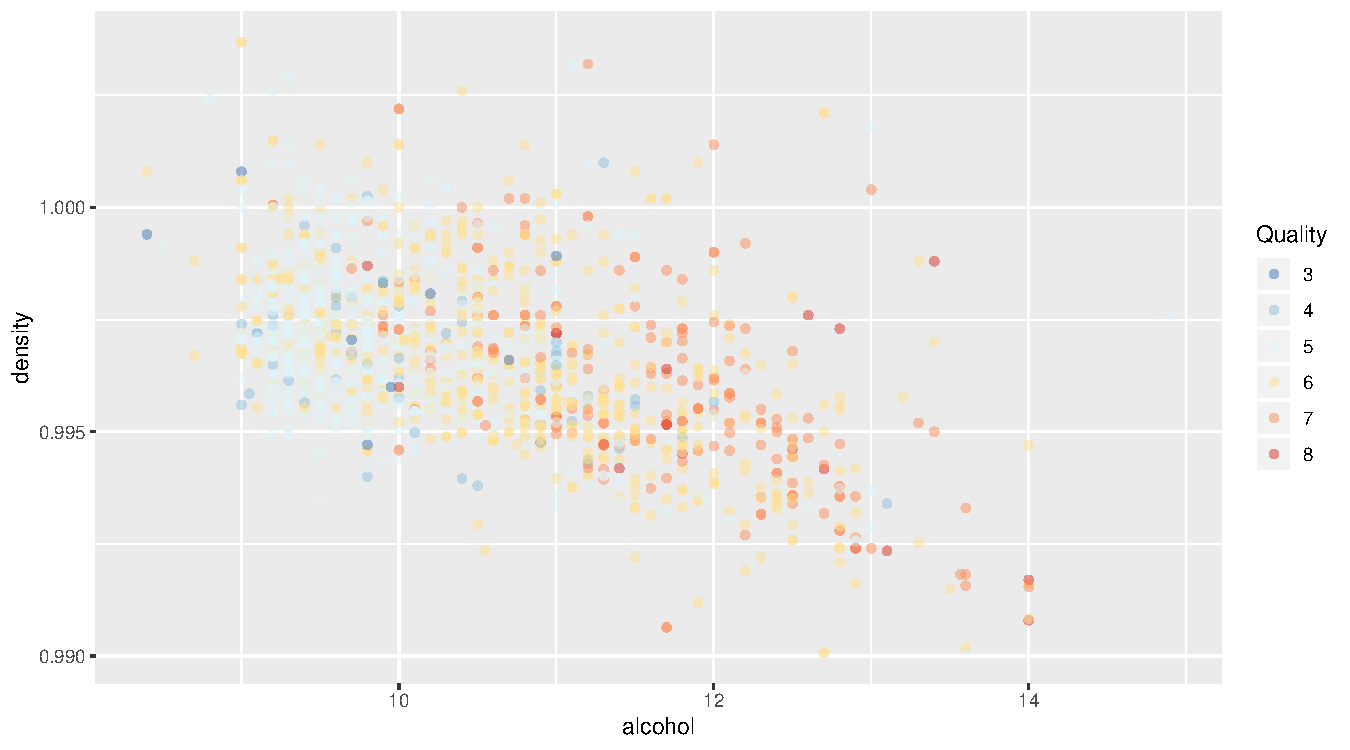
\includegraphics{RedWineQuality-Project6_files/figure-latex/Multivariate_Plots-1.pdf}

\begin{quote}
From the scatterplot above we can observe the inverse relation between
density and alcohol, when density increases the alcohol decreases. we
can also see that the quality of red wine is assosicated with high level
of alcohol and lower density values which proves previous investigation.
\end{quote}

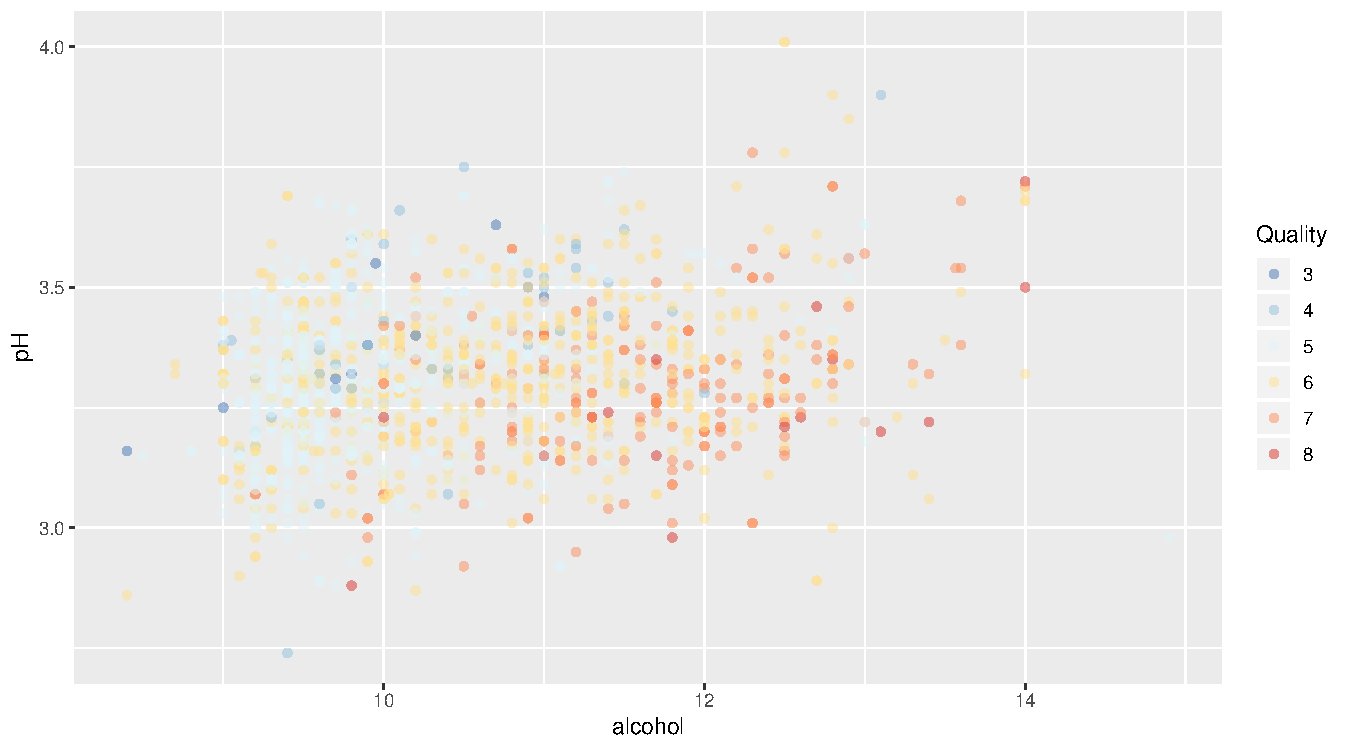
\includegraphics{RedWineQuality-Project6_files/figure-latex/unnamed-chunk-14-1.pdf}

\begin{quote}
The above scatterplot shows a weak relationship between pH value and
alcohol most samples scores between 3 to 3.5 pH and associated with 10
alcohol value and the increase in alcohol associated with more quality
rates.
\end{quote}

\hypertarget{multivariate-analysis}{%
\section{Multivariate Analysis}\label{multivariate-analysis}}

\hypertarget{talk-about-some-of-the-relationships-you-observed-in-this-part-of-the-1}{%
\subsubsection{\texorpdfstring{Talk about some of the relationships you
observed in this part of the\\
}{Talk about some of the relationships you observed in this part of the }}\label{talk-about-some-of-the-relationships-you-observed-in-this-part-of-the-1}}

investigation. Were there features that strengthened each other in terms
of\\
looking at your feature(s) of interest?

The Density, alcohol and quality scatterplot strenghtened the previous
observed data from the bivariate section and showed how both of those
two factors contributed in the red wine quality rating.

\hypertarget{were-there-any-interesting-or-surprising-interactions-between-features}{%
\subsubsection{Were there any interesting or surprising interactions
between
features?}\label{were-there-any-interesting-or-surprising-interactions-between-features}}

The pH value of the red wine has no effect on the quality results nor
even has a clear relationship with alcohol which is surprising.

\begin{center}\rule{0.5\linewidth}{\linethickness}\end{center}

\hypertarget{final-plots-and-summary}{%
\section{Final Plots and Summary}\label{final-plots-and-summary}}

\hypertarget{plot-one}{%
\subsubsection{Plot One}\label{plot-one}}

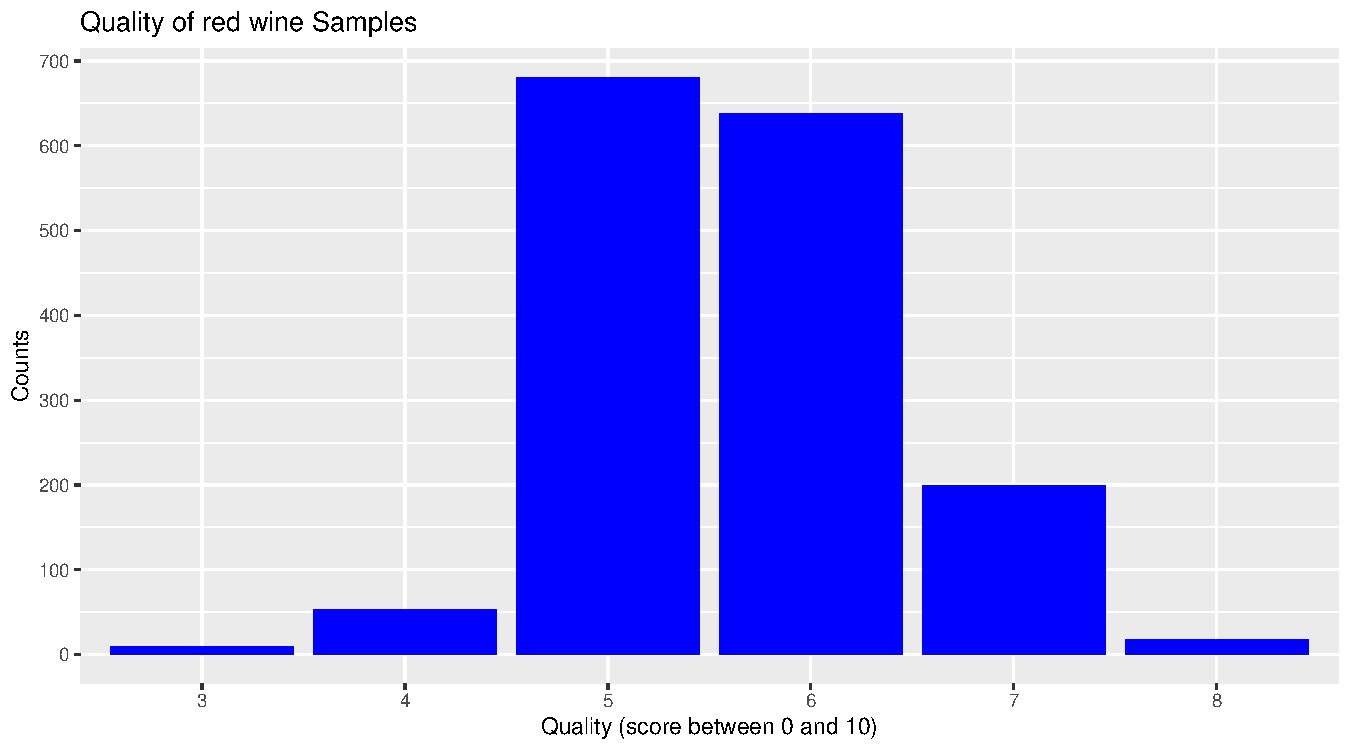
\includegraphics{RedWineQuality-Project6_files/figure-latex/Plot_One-1.pdf}

\hypertarget{description-one}{%
\subsubsection{Description One}\label{description-one}}

\begin{quote}
The quality histogram shows that the majority of wine samples are rated
5 or 6 while few samples are rated 1 and 8 and no sample rated above 8
nor less than 3.
\end{quote}

\hypertarget{plot-two}{%
\subsubsection{Plot Two}\label{plot-two}}

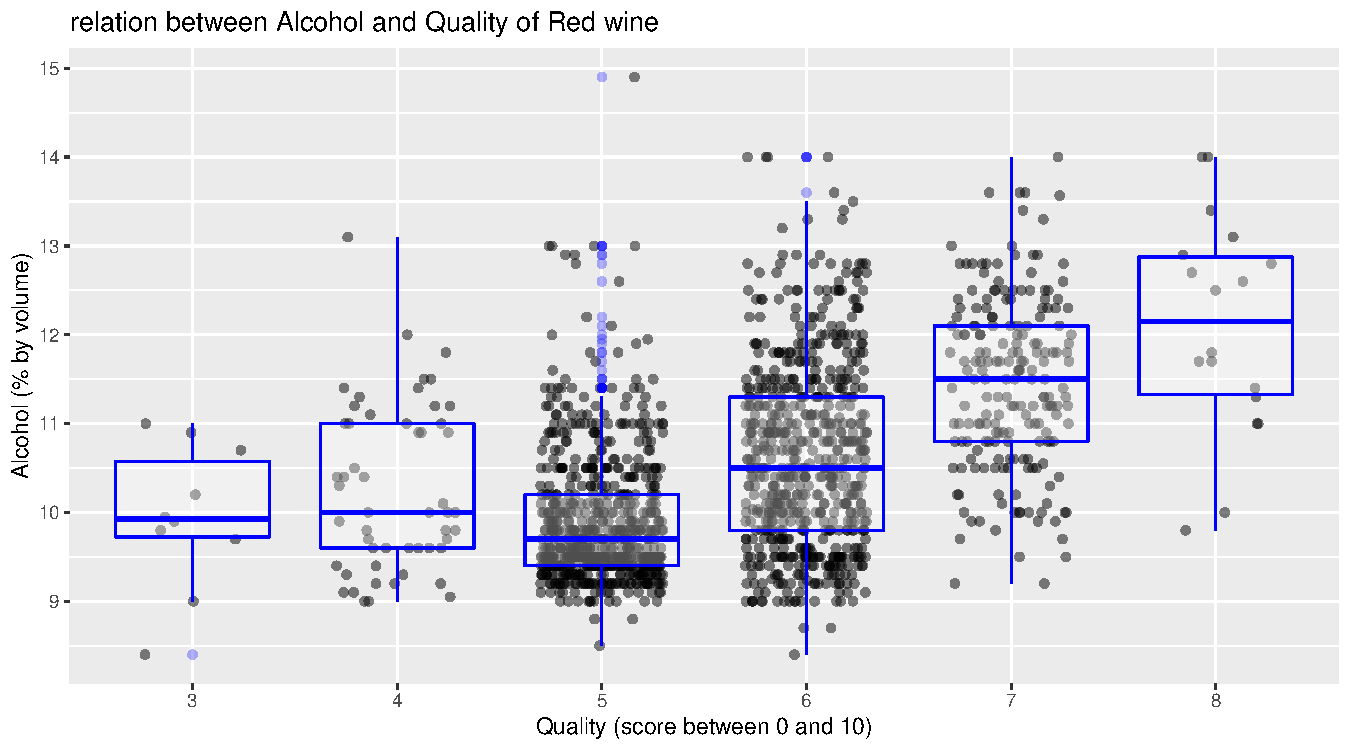
\includegraphics{RedWineQuality-Project6_files/figure-latex/Plot_Two-1.pdf}

\hypertarget{description-two}{%
\subsubsection{Description Two}\label{description-two}}

\begin{quote}
The plot above shows the relation between alcohol and the quality of red
wine, and we can observe that the quality increases when alcohol
increases.
\end{quote}

\hypertarget{plot-three}{%
\subsubsection{Plot Three}\label{plot-three}}

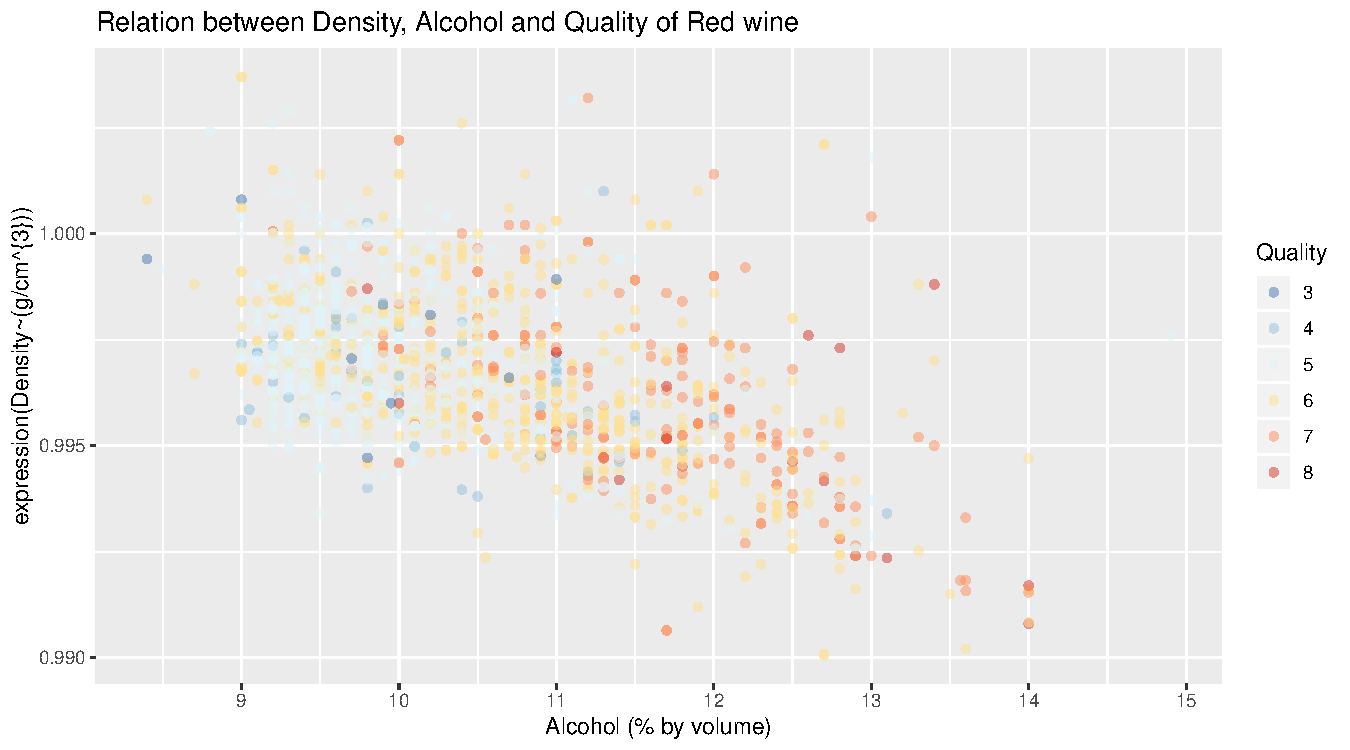
\includegraphics{RedWineQuality-Project6_files/figure-latex/Plot_Three-1.pdf}

\hypertarget{description-three}{%
\subsubsection{Description Three}\label{description-three}}

\begin{quote}
The above scatterplot shows a weak relationship between pH value and
alcohol most samples scores between 3 to 3.5 pH and associated with 10
alcohol value and the increase in alcohol associated with more quality
rates.
\end{quote}

\begin{center}\rule{0.5\linewidth}{\linethickness}\end{center}

\hypertarget{reflection}{%
\section{Reflection}\label{reflection}}

\begin{quote}
The Red wine database contains around 1600 sample of red wine data and
all of their chemical combinations, with these data we performed a high
level data analysis to understand how much every variable of these
chemicals contribute the most in each sample quality.
\end{quote}

\begin{quote}
Our observation from these data that some variables has big impact on
the quality rating and some other not for instance, alcohol showed a
propotional relationship toward the quality whenever the alcohol
increases the quality increases. Another factor which has big impact on
quality is the density of the red wine sample it has inverse
relationship with the quality, when the density increases the quality
decreases and the alcohol value as well.
\end{quote}

\begin{quote}
For the pH value is surprising since it does not have any impact on the
quality our plots shows no matter high or less the pH value the quality
remain the same.
\end{quote}

\begin{quote}
Our analysis is limited to the small data set we observed our data from
as well as the information we have for each sample as well as using
lineear regression model only.
\end{quote}

\begin{quote}
Furthermore, for future analysis we might use logestic regression
analysis for better analysing the red wine quality.
\end{quote}


\end{document}
